\newpage
\section{Testowanie}
Testy automatyczne są bardzo ważną częścią każdej aplikacji. Pozwalają one w łatwiejszy sposób wprowadzać zmiany do aplikacji, mając większą pewność, że zmiany nie wprowadziły niepożądanych błędów do kodu źródłowego. Dodatkowo podczas procesu pisania kodu aplikacji, dzięki takim testom programista jest w stanie w łatwy sposób sprawdzić poprawność rozwiązań w wielu różnych sytuacjach.

Aplikacja została przetestowana na trzy różne sposoby:
\begin{enumerate}
  \item Jednostkowo
  \item Integracyjnie
  \item Z użyciem wizualnej regresji
\end{enumerate}

\subsection{Testowanie jednostkowe aplikacji klienckiej}
Testowanie jednostkowe pozwala w prosty sposób przetestować poszczególne komponenty aplikacji w izolacji. Komponenty w bibliotece React to zwykłe funkcje, więc można by pomyśleć, że możemy je testować jak funkcje, jednak jest kilka rzeczy, o których musimy pamiętać.

\subsubsection{Testowanie komponentów React}
Jednym z powodów, dla którego trudno jest testować komponenty jak zwykłe funkcje, jest to, że komponenty mogą posiadać stan. Jak widać na wydruku \ref{lst:reactCounterCode}, używając funkcji \emph{React.useState} dołączamy do funkcji stan, który może się różnić przy różnych wywołaniach danego komponentu. Z tego powodu kolejne wywołania tej samej funkcji mogą zwracać inny wynik.

Kolejnym powodem, dla którego trudno by było przetestować komponent, bazując tylko i wyłącznie na jego zwróconym wyniku, jest to, że wartością zwracaną przez komponent jest zwykły obiekt, który reprezentuje część wirtualnego DOM-u. Natomiast my jako programiści interpretujemy tę część wirtualnego DOM-u jako prawdziwe elementy przeglądarki, dlatego asercje, które sprawdzałyby poprawność wirtualnego DOM-u mogłyby być nieczytelne i trudne w utrzymaniu.

Dodatkowo komponenty mogą używać interfejsu przeglądarki, więc aby w całości przetestować komponent, musimy być w stanie też sprawdzić, jak komponenty wchodzą w interakcje z przeglądarką.

Aby móc poprawnie i efektywnie przetestować jednostkowo komponenty aplikacji zostały użyte dwie biblioteki: \emph{react-testing-library} \cite{ref_rtl_doc} oraz \emph{Jest} \cite{ref_jest_doc}.

\subsubsection{Jest} \emph{Jest} to biblioteka, która udostępnia programiście interfejs, który umożliwia testowanie kodu napisanego w języku Javascript, w szczególności komponenty React. Aby zasymulować środowisko przeglądarki,
\emph{Jest} używa sztucznego środowiska o nazwie \emph{jsdom}, dzięki któremu programista może testować kod w środowisku, w którym kod Javascript będzie wykonywany, czyli w przeglądarce. Biblioteka \emph{Jest} została stworzona przez Facebook'a i jest nadal rozwijana.

\emph{Jest} posiada dużo funkcji, które ułatwiają testowanie kodu Javasrcipt.
\begin{description}
  \item[Interfejs do tworzenia asercji] \hfill \\ \emph{Jest} udostępnia prosty i zrozumiały interfejs, dzięki któremu możemy tworzyć bardzo czytelne testy. Nazwy asercji są bardzo intuicyjne i czyta się je jak prawdziwe zdania w języku angielskim.
  \begin{addmargin}[6mm]{0mm}
  \begin{lstlisting}[
      numbers=left,
      firstnumber=1,
      caption={Przykład testu napisanego w bibliotece \emph{Jest}},
      aboveskip=10pt
  ]
  test('funkcja powinna byc zawolana', () => {
    // zakladajac
    let funkcja = jest.fn();

    // kiedy
    funkcja();

    // wtedy
    expect(funkcja).toEqual(funkcja);
    expect(funkcja).toHaveBeenCalledTimes(1);
  })
  \end{lstlisting}
  \end{addmargin}


  \vspace{0.4cm}

  \item[Równoległe uruchamianie testów] \hfill \\ \emph{Jest} pozwala na uruchamianie testów jednocześnie w wielu wątkach, przez co testy wykonują się nawet kilka razy szybciej, niż gdyby odpalało się je pojedynczo.

  \vspace{0.4cm}

  \item[Migawki] \hfill \\ \emph{Jest} udostępnia interfejs, dzięki któremu możemy tworzyć tzw. migawki (ang. snapshots). Migawki są techniką pozwalającą testować zmiany, które mogły nastąpić pomiędzy kolejnymi uruchomieniami testów.
  \begin{addmargin}[6mm]{0mm}
  \begin{lstlisting}[
      numbers=left,
      firstnumber=1,
      caption={Przykład testu migawkowego},
      aboveskip=10pt
  ]
  function funkcjaDoMigawki() {
    return '<div>Witaj swiecie!</div>';
  }

  test('funkcja powinna zwracac poprawny wynik', () => {
    expect(funkcjaDoMigawki).toMatchSnapshot();
  })
  \end{lstlisting}
  \end{addmargin}
  Powyżej w teście widzimy, że funkcja \emph{funkcjaDoMigawki} zwraca tag \emph{div} z tekstem w środku. W teście moglibyśmy sprawdzić zawartość zwróconej wartości przez funkcję, lecz wymagałoby to ręcznego wpisania wartości w asercji. W przykładzie jest to tylko jedna linijka, ale w przypadku komponentów React, które mogą zwracać nawet kilkadziesiąt linijek, wpisywanie ręczne zwracanej wartości mogłoby się okazać dosyć trudnym zadaniem.

  Migawki rozwiązują ten problem. \emph{toMatchSnapshot} podczas pierwszego uruchomienia zapamiętuje wartość zwróconą przez funkcję, a przy następnych uruchomieniach testu sprawdza, czy wynik zgadza się z wynikiem z poprzedniego uruchomienia. Jeżeli te dwie wartości nie będą się zgadzać, \emph{Jest} zwróci programiście, że test nie przeszedł. W takiej sytuacji programista może zaakceptować nowy wygląd migawki lub poprawić błąd, jeżeli zmiana była niezamierzona. Takie testy są właśnie stworzone po to, aby nie wprowadzać niepożądanych zmian do kodu aplikacji.

\subsubsection{React-testing-library} React-testing-library natomiast rozwiązuje problem czytelności i łatwości testowania komponentów. Dzięki tej bibliotece jesteśmy w stanie testować zachowanie komponentów, używając do tego bardzo prostego interfejsu, który pozwala na wykonywanie takich operacji jak:
\begin{itemize}
  \item łatwe tworzenie komponentów w wirtualnym środowisku
  \item wykonywanie akcji użytkownika np. klikanie, najeżdżanie myszką itp.
  \item łatwe wyszukiwanie elementów i sprawdzanie ich stanu lub atrybutów
\end{itemize}


\end{description}
  \begin{addmargin}[6mm]{0mm}
  \begin{lstlisting}[
      numbers=left,
      firstnumber=1,
      caption={Przykład testu jednostkowego przy użyciu React-testing-library},
      aboveskip=10pt
  ]
    test('gdy nazwa wydatku jest za dluga powinien pojawic sie blad', () => {
    // given
    const { getByLabelText, queryByText } = render(<FormularzWydatku />);

    // when
    const poleZNazwa = getByLabelText('Nazwa wydatku');

    await userEvent.type(poleZNazwa, 'x'.repeat(51));

    // then
    const blad = queryByText(
      "Pole nie moze miec wiecej niz 50 znakow."
    );

    expect(blad).toBeInTheDocument();
  });
  \end{lstlisting}
  \end{addmargin}
  Powyżej w teście możemy zauważyć, że symulujemy wpisywanie do pola \emph{Nazwa wydatku} 51 znaków, a następnie sprawdzamy, czy w komponencie wyświetlił się odpowiedni błąd. Dzięki takim testom komponentów możemy w łatwy sposób przetestować zachowanie komponentów w wielu różnych scenariuszach.

Testowanie jednostkowe ma natomiast kilka ograniczeń:
\begin{itemize}
  \item nie pozwala sprawdzać integracji aplikacji z serwisami zewnętrznymi np. komunikacji z serwerem
  \item jako że Jsdom tylko symuluje środowisko przeglądarki, w aplikacji mogą pojawiać się błędy, które pojawiają się w prawdziwej przeglądarce. Takich błędów testy jednostkowe nie są w stanie wykazać
\end{itemize}

\subsection{Testowanie integracyjne aplikacji klienckiej}
Testowanie integracyjne pozwala rozwiązać te wyzwania, które wystąpiły przy testowaniu jednostkowym.

Do testów integracyjnych użyłem biblioteki o nazwie \emph{Cypress.io} \cite{ref_cypress_doc}. Biblioteka ta pozwala pisać testy, które potem są wykonywane w prawdziwej instancji przeglądarki. Cypress udostępnia interfejs, dzięki któremu możemy wykonywać akcje użytkownika (np. wpisywanie tekstu, klikanie itp.). Pozwala także sprawdzać poprawne działanie zewnętrznych serwisów, jak i komunikację z nimi.

  \begin{addmargin}[6mm]{0mm}
  \begin{lstlisting}[
      numbers=left,
      firstnumber=1,
      caption={Przykład testu integracyjnego z użyciem biblioteki Cypress},
      aboveskip=10pt
  ]
  it('wydatek powinien sie usunac', () => {
    // register
    cy.visit('/login');
    logIn(1);

    // create new expense
    cy.contains('Przykladowy opis zmieniony').click();
    cy.contains('Usun').click();
    cy.contains('OK').click();

    cy.contains('Przykladowy wydatek zmieniony').should('not.exist');
    cy.contains('Przykladowy opis zmieniony').should('not.exist');
  });
  \end{lstlisting}
  \end{addmargin}
  Powyżej przedstawiony jest przykładowy test integracyjny aplikacji. Przy użyciu interfejsu Cypress możemy sterować przeglądarką i tworzyć testy, które symulują akcje użytkownika w instancji przeglądarki.

Cypress udostępnia też podgląd testów \emph{na żywo}. Dzięki temu, gdy test będzie nieudany, możemy w łatwy sposób stwierdzić, w którym miejscu aplikacji wystąpił błąd. Na rysunku \ref{fig-cypress} widzimy przykład testu w panelu Cypress. Po lewej stronie są wyświetlane wszystkie komendy wywoływane przez bibliotekę Cypress, a po prawej stronie wynik tych akcji w przeglądarce.

\begin{figure}
    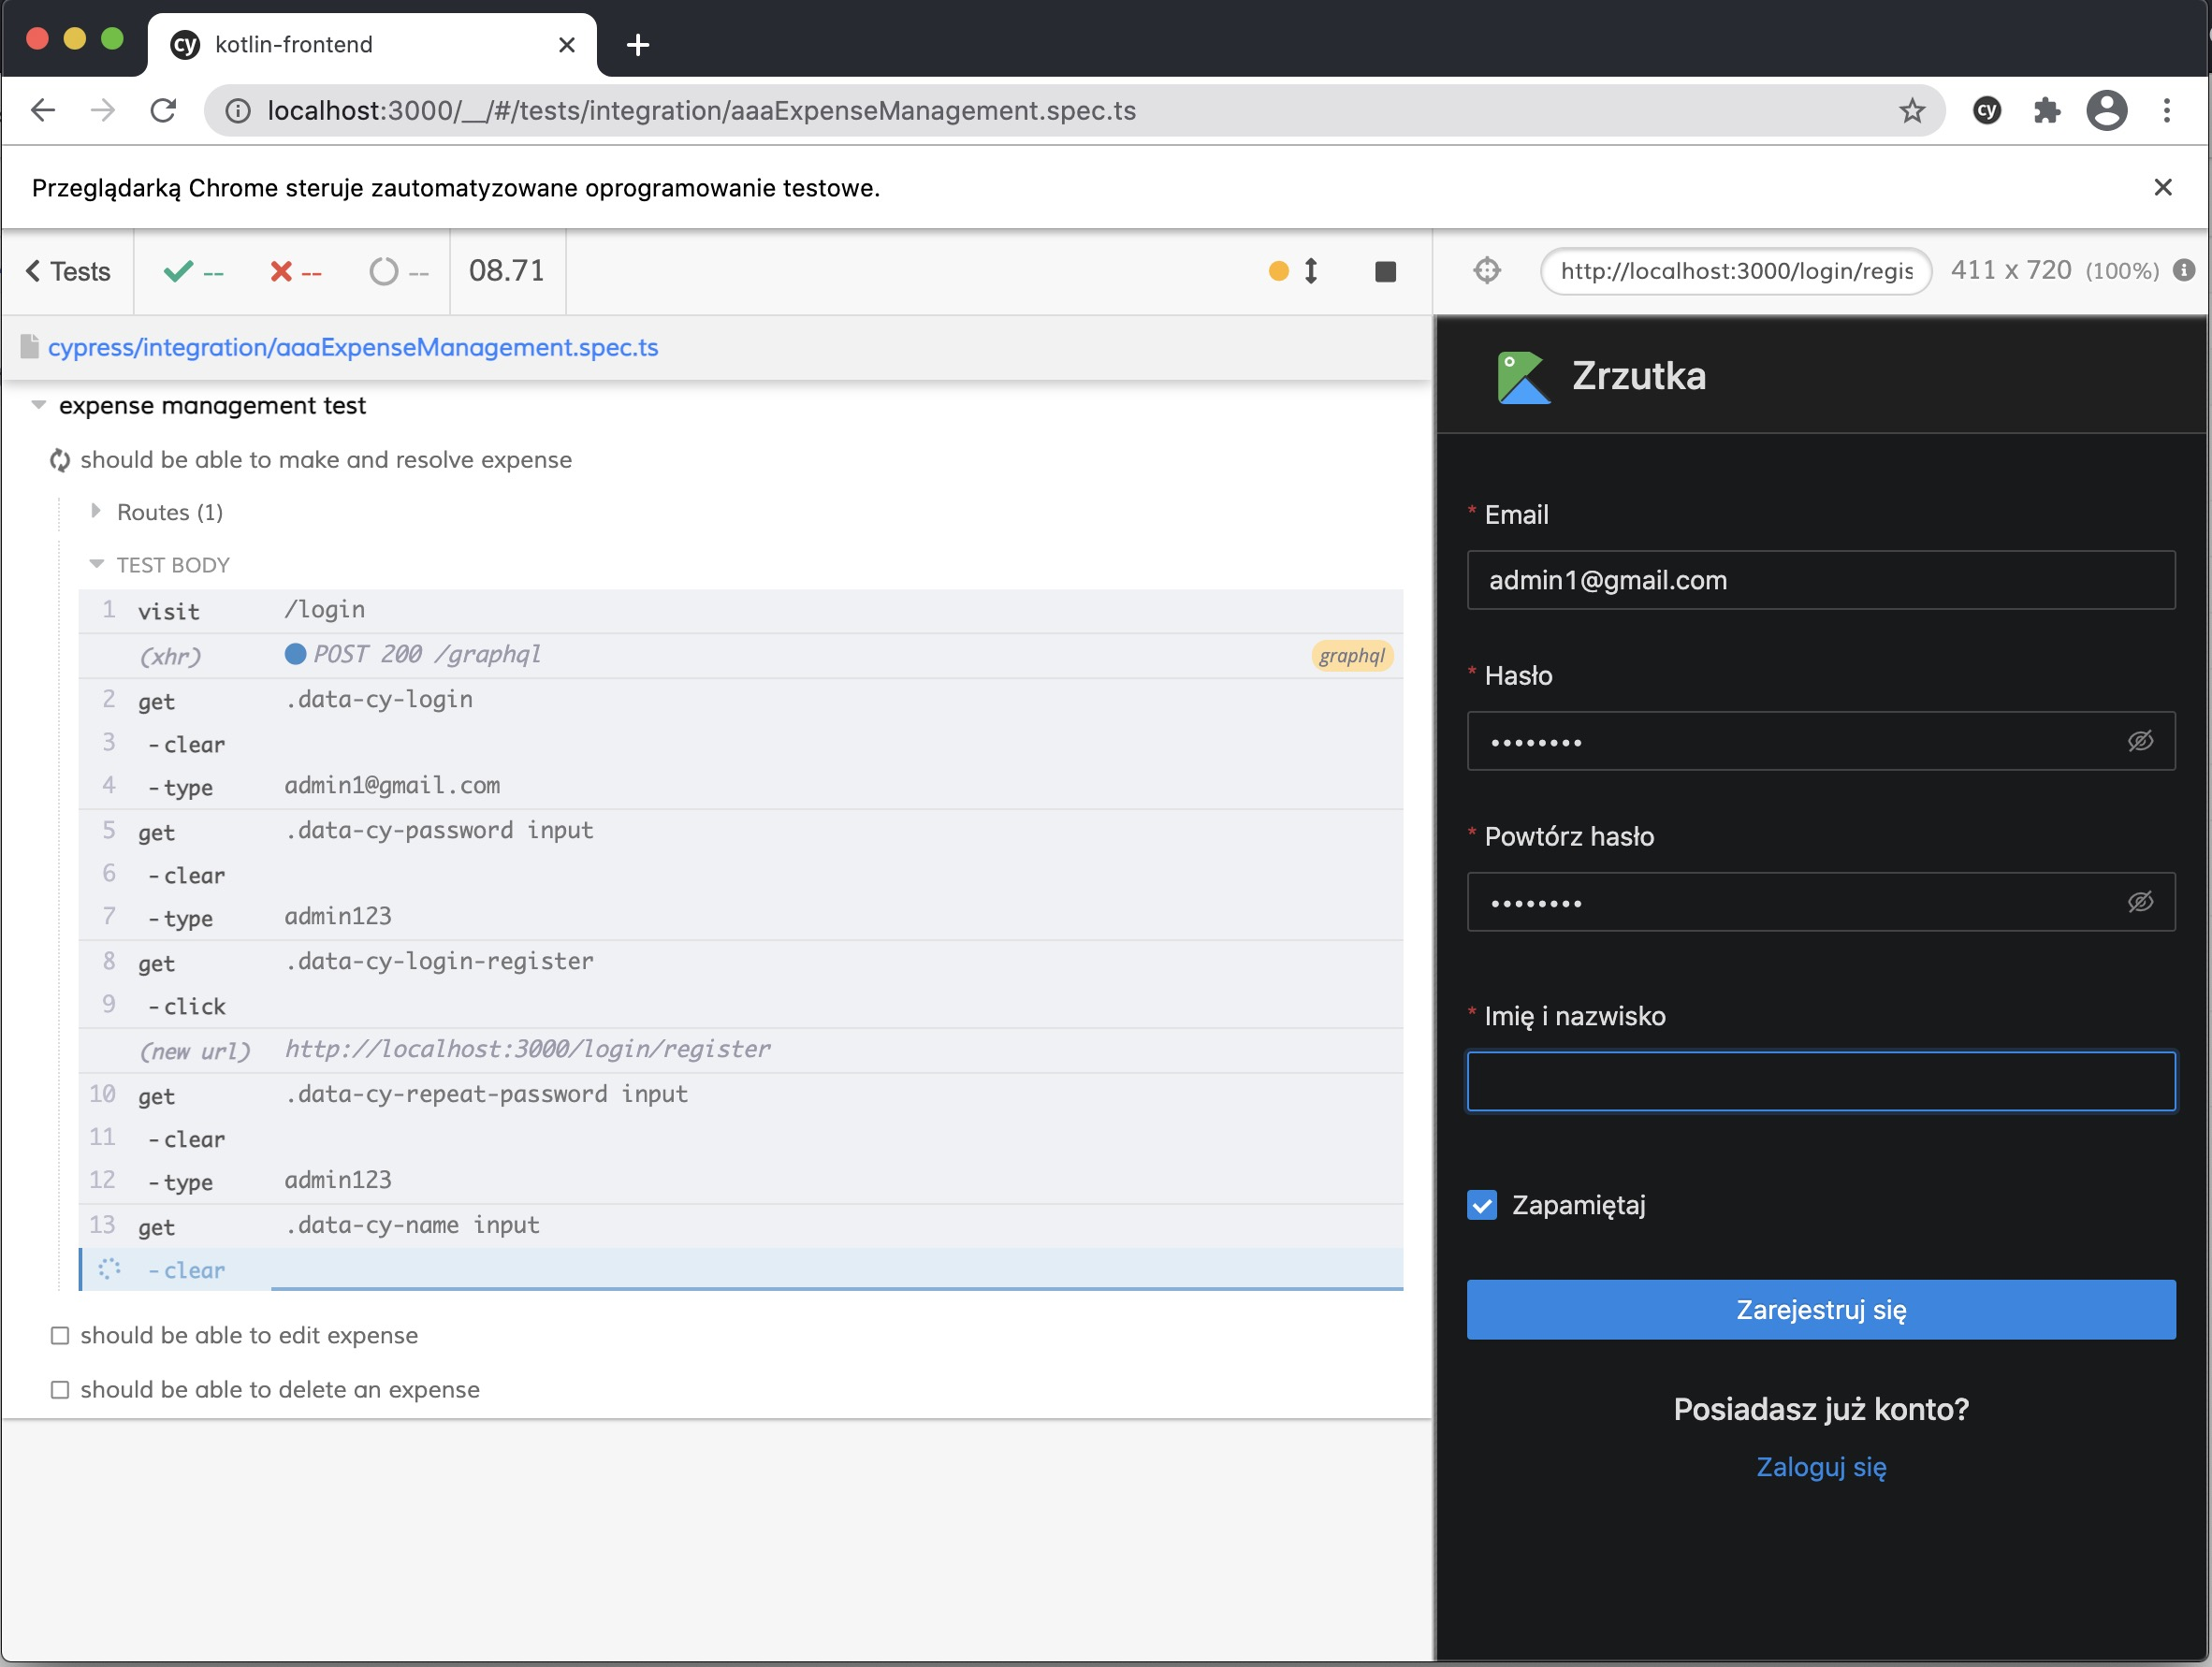
\includegraphics[width=\textwidth]{cypress-imape.jpg}
    \caption{Panel Cypress.io} \label{fig-cypress}
\end{figure}

\subsection{Testy wizualnej regresji aplikacji klienckiej}
Testy wizualnej regresji zapewniają wizualną poprawność interfejsu użytkownika. Dzięki nim mogłem programowo symulować sytuacje biznesowe, a następnie przy pomocy biblioteki Cypress.io robić zrzuty ekranu. Testy wizualnej regresji działają podobnie jak testy migawkowe, tylko zamiast zapamiętywania wartości zwróconej przez funkcję Cypress zapamiętuje zrzut ekranu przeglądarki. Gdy pierwszy zrzut ekranu aplikacji został zrobiony podczas pierwszego uruchomienia testu, każde następne uruchomienie tego samego testu będzie robiło kolejny zrzut, a następnie porównywało z poprzednim. W taki sposób możemy sprawdzać, czy po zmianach w kodzie nie nastąpiła niepożądana zmiana w wyglądzie aplikacji. Jeżeli takie dwa zrzuty się różnią, test wyświetli komunikat o błędzie, a następnie wyświetli różniące się zrzuty ekranu i wyróżni wszystkie różniące się piksele obu zdjęć. Jeżeli natomiast zmiana wyglądu była zamierzona, programista może zaakceptować zmiany w teście i od tego momentu w następnych testach porównywać z nowym wyglądem.

% todo change screen to have new name and logo
\begin{figure}
    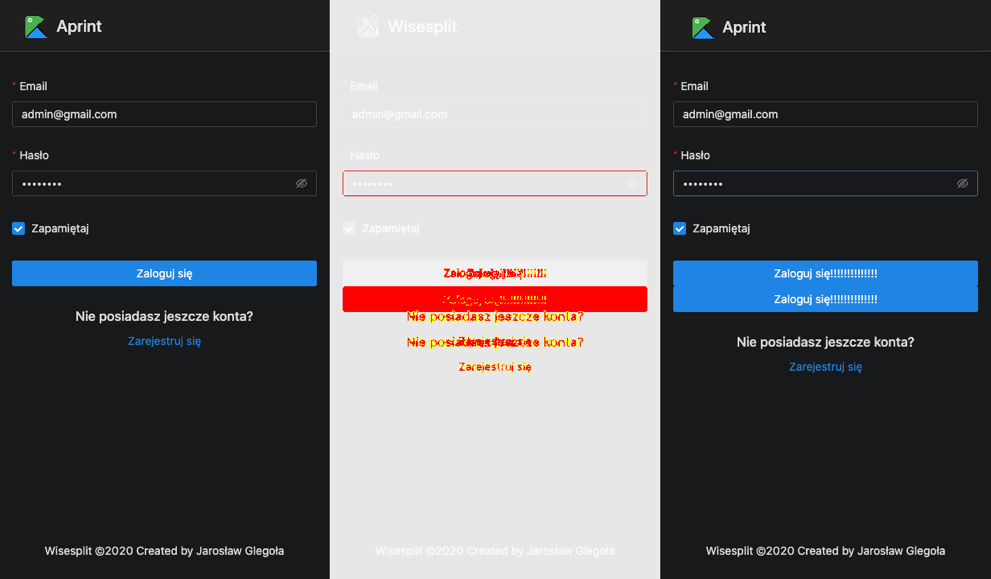
\includegraphics[width=\textwidth]{wisual-regression.png}
    \caption{Przykład wyniku nieudanego testu wizualnej regresji} \label{fig-cypress-vr}
\end{figure}


\subsection{Testy integracyjne aplikacji serwerowej}
Aplikację serwerową testowałem głównie integracyjnie. Do pisania testów wybrałem język Groovy i bibliotekę Spock w środowisku JUnit. Testy integracyjne serwera nie różnią się w dużej mierze od testów integracyjnych aplikacji klienckiej. Jedyną różnicą jest to, że nie posiadamy wizualnej części. Testy integracyjne testują wszystkie elementy aplikacji serwerowej: zapytania klienckie, logikę biznesową oraz integrację z bazą danych.
